\documentclass[a4paper,12pt]{article} % format of document

\usepackage[english,russian]{babel} % add eng,rus(base) package
\usepackage[T1,T2A]{fontenc}        % add eng,rus encoding support
\usepackage[utf8]{inputenc}         % add UTF8 support
\usepackage{soul}         	    % add l a t e r s p a c i n g
\usepackage{longtable}         	    % To display tables on several pages
\usepackage{booktabs}         	    % For pretter tables
\usepackage{enumitem}         	    % advanced list support

\usepackage{amsmath, amsfonts, amssymb, amsthm, mathtools} % add math support

\usepackage{geometry}  % add document's fields correction support
\geometry{top=25mm}    % top field
\geometry{bottom=30mm} % bottom field
\geometry{left=20mm}   % left field
\geometry{right=20mm}  % right field

\linespread{1}               % length between str
\setlength{\parindent}{20pt} % red str
\setlength{\parskip}{12pt}   % length between paragraphs

\usepackage[backend=biber, style=authoryear-icomp]{biblatex} % add bibliography support
\addbibresource{$HOME/latex-templates/biblio.bib}            % path to bibliography base
\usepackage{csquotes}                                        % advanced facilities for inline and display quotations

\usepackage{indentfirst} % first paragraph with red str

% Must be the last command into the preamble of document.
\usepackage{hyperref} % All references in document turn into hyperlinks
\hypersetup{
unicode=true,      % юникод в названиях разделов pdf
colorlinks=true,   % цветные ссылки вместо ссылок в рамках
linkcolor=blue,    % внутренние ссылки
citecolor=green,   % ссылки на библиографию
filecolor=magneta, % ссылки на файлы
urlcolor=blue,     % ссылки на url
}
 % here is document's settings for russian
%\input{$HOME/studyproject/universe/history/preamble-beamer-eng.tex} % here is document's settings for english


\title{Эссе на тему: Иван III --- Первый государь всея Руси}
\author{Немков Николай Максимович СМ4-11}

\date{30.10.2023}
%\logo{
\includegraphics[width=1cm]{images/logo}}

\begin{document}

\maketitle
\begin{center}
Московски Государственный Технический Университет им. Н.Э. Баумана

Преподаватель: Щербакова Ольга Михайловна
\end{center}
\newpage
\tableofcontents

\newpage
\section{Вступление}
			Фигура великого князя Ивана III Васильевича (1440-1505г) незаслужанно мало известно людям. Между тем одного перечисления сделанного им хватит, что бы поставить его в ряд исторических личностей первой велечины.


    \begin{center}
	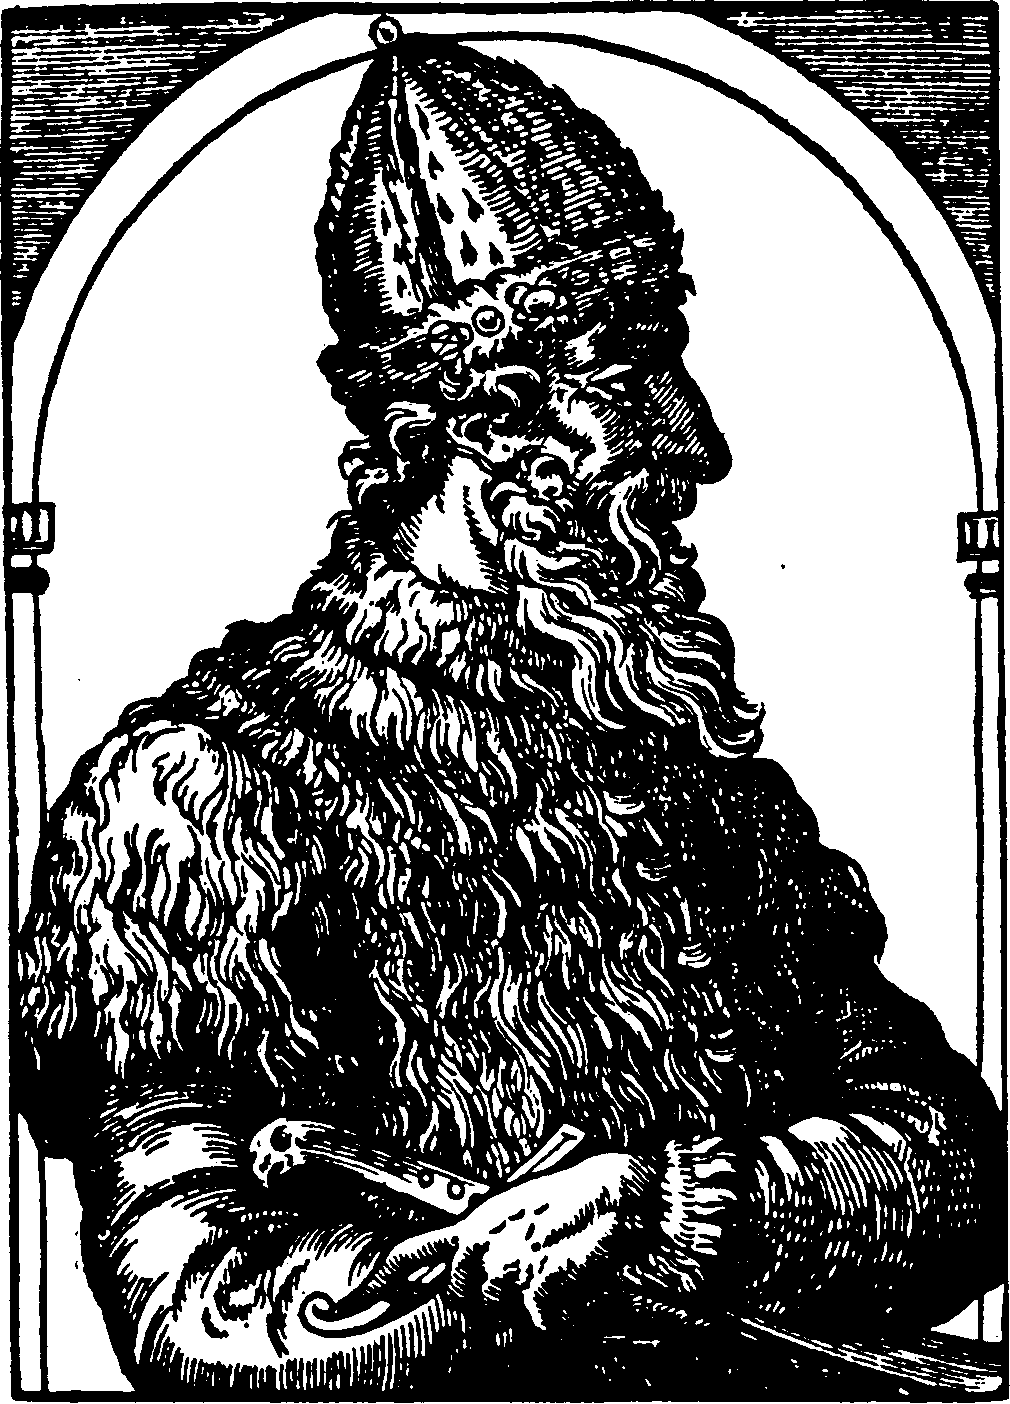
\includegraphics[width=0.5\textwidth]{images/ivan2-1}
    \end{center}

\newpage
\section{Основная часть}

	В 22 года Мван Васильевич начал управлять Москвой один. Толково, осмотрительно, дальновидно. И все вспоминает завет своего покойного батюшки:

	-- Дело предков своих продолжай. Собирай Русские земли вокруг Москвы. И крепко держите земли в руках.



	За сороколетний период правления Иван III завершил объединение разрозненых княжеств и земель, из которых выросло новое единое Русское государство.

	Присоединился к Москве Ярославль, Великий Новгород, покорился Пермский край, продали Ивану Васильевичу свои земли ростовские князья.


			Старое самоназвание страны --- Русь --- продолжало использоваться, но именно в правление Ивана III появляется сохранившееся до сих пор -- Россия

			Еще одним символом восходящим к той эпохе, стал государственный герб с изображением двуглавого орла.
    \begin{center}
	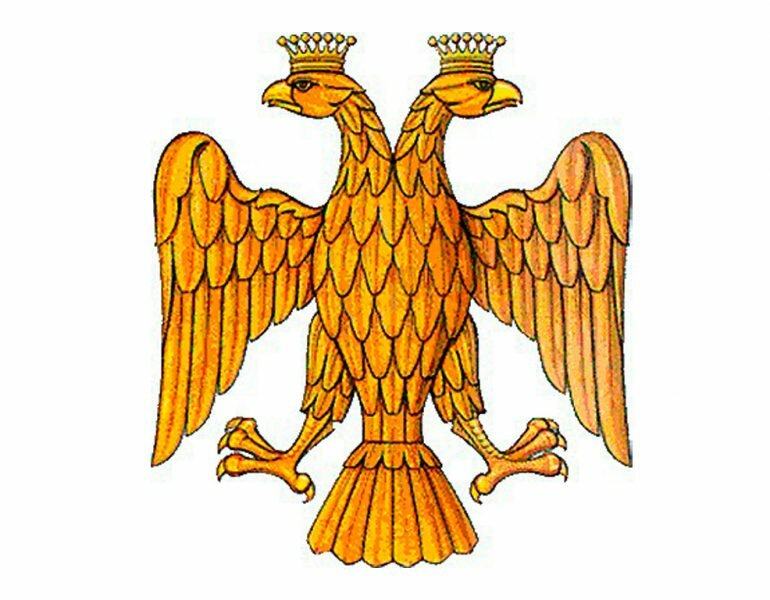
\includegraphics[width=0.5\textwidth]{images/ivan2-2}
    \end{center}



\newpage
	При Иване III был принят первый в истории России Судебник.

    \begin{center}
	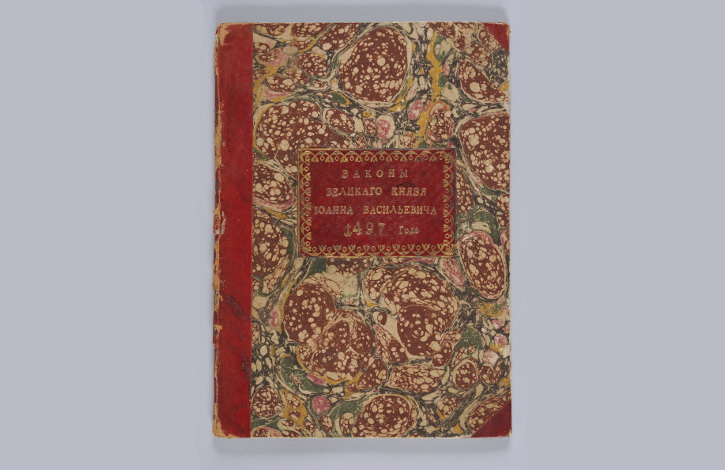
\includegraphics[width=0.5\textheight]{images/ivan2-3}
    \end{center}




	В 1497 году явились в Кремлевские полаты бояре и с поклоном протянули Ивану Васильевичу пухлую книгу в кожаном переплете. "Судебник" --- золотыми буквами было написанно на обложке. Медленно, осторожно государь перелестал страницы. все законы тут собраны: икак наследство делить, и как за воровство наказывать, и как подати платить. Будут отныне на Руси народ судить по законам.



\section{Заключение}
	Великий князь Иван III в целом завершил объединение русских земель, выполнив тем самым основную задачу, стоявшую перед потомками Ивана Калиты. Второмым важным его достижением стало избавление от ордынского ига. Особенно ценно, что Иван Васильевич сам поставил перед собой эту задачу.

\newpage
\section{Список литературы}
	1. Воробьев А.В. Великий князь Иван III Васильевич \url{https://biblioclub.ru/index.php?page=book&id=456103}


	2. Российское вокнно-историческое общество Цари-полководцы \url{https://biblioclub.ru/index.php?page=book&id=456270}

	3. Мартиросова М.А. Иван III Государь всея Руси \url{https://www.iprbookshop.ru/51320.html}

\end{document}
